\documentclass{article}

\usepackage[utf8]{inputenc}
\usepackage{mathtools}
\usepackage{amssymb}
\usepackage{amsmath}
\usepackage{amsthm}
\usepackage{enumitem}
\usepackage{tikz}
\usetikzlibrary{patterns}



\title{Discrete Geometrie I - Assignment 02}
\date{}
\author{Viet Duc Nguyen (395220)\\
    \underline{vd.nguyen96@gmail.com}
}



\begin{document}

\maketitle

\section*{Exercise 1}
\begin{enumerate}[label=(\alph*)]
    \item Let $n \in \mathbb N$ be arbitrary, and let $e_i$ denote the $i$-th unit vector in $\mathbb R^n$. Consider the hyperplanes 
    \begin{align*}
        A_i &= \{ x \in \mathbb R^n : \langle x,e_i \rangle = 0 \}, \quad i = 1,...,n \\
        A_{n+1} &= \{ x \in \mathbb R^n: \langle x,\sum_{i=1}^ne_i \rangle = 42 \}
    \end{align*}
    \begin{itemize}
        \item It holds $\bigcap_{i=1}^{n+1} A_i = \emptyset$: we see that $$\bigcap_{i=1}^{n+1} A_i = \left(\bigcap^n_{i=1} A_i\right) \cap A_{n+1} = \{0\} \cap A_{n+1} = \emptyset.$$

        \item $A_i$ is convex for all $i=1,...,n+1$, since affine linear spaces are convex and $A_i$ is the solution space of a linear equation, which is an affine linear space.
        
        \item $\bigcap_{j=1}^n A_{i_j} \neq \emptyset:$ For any $A_{i_1},...,A_{i_n}$, each $A_{i_j}$ represents a hyperplane, whose normal vector is not colinear to the other normal vectors. Therefore, $\bigcap_{j=1}^n A_{i_j}$ defines a system of $n$ linear equations with $n$ variables that has exactly one solution, for the normal vectors are linear independent. Thus, $\bigcap_{j=1}^n A_{i_j}$ is nonempty.
    \end{itemize}
    
    

    \item Let $d \in \mathbb N_{\geq 3}$. Consider the sets $A_i = \{ (x_1,...,x_d) \in \mathbb R^d : x_2,...,x_{d} \geq 0, x_1 \geq i \}$. Then, $(A_i)_{i \in \mathbb N}$ is a family of convex sets, and $\bigcap_{i \in \mathbb N} A_i = \emptyset$. Furthermore, any sets $A_{i_1},...,A_{i_{d+1}}$ share a common point since $(i,0,...,0) \in \bigcap_{j=1,...,d+1} A_{i_j}$ for $i = \max_{j=1,...,d+1}\{i_j \}$.
\end{enumerate}



\subsection*{Exercise 2}

\begin{itemize}
    \item \textbf{Closed under multiplication:} Let $f,g \in \mathcal C(\mathbb R^d)$. Then, $f = \sum_{i=1}^{n}\lambda_i [A_i]$ and $g = \sum_{i=1}^m \mu_i [B_i]$, where $A_i$ and $B_i$ are closed convex sets in $\mathbb R^d$. We would like to prove that $f \cdot g$ is a linear combination of indicator functions of closed convex sets. In that case, $f \cdot g \in \mathcal C(\mathbb R^d)$. So,
    
    \begin{align*}
        f \cdot g = \left(\sum_{i=1}^{n}\lambda_i [A_i]\right) \cdot \left(\sum_{i=1}^m \mu_i [B_i]\right) &= \sum_{i=1}^{n}\left(\lambda_i[A_i] \cdot  \sum_{j=1}^m \mu_j [B_j] \right) \\
        &= \sum^n_{i=1}\sum^m_{j=1}\left(\lambda_i[A_i]\mu_j[B_j]\right) \\
        &= \sum^n_{i=1}\sum^m_{j=1} \lambda_i\mu_j[A_i \cap B_j].
    \end{align*}
    For each $i,j$ the set $A_i \cap B_j$ is closed and convex. Thus, $f\cdot g$ is indeed a linear combination of indicator functions of closed convex sets.

    \item $\mathcal C(\mathbb R^d)$ is not a finite dimensional real vector space. Assume it would be. In that case, there exists a basis $\left([A_1],...,[A_n]\right)$ of $\mathcal C(\mathbb R^d)$. Furthermore, we can assume that each $A_i$ and $A_j$ are pairwise disjoint for $i,j = 1,...,n$. If there would be $A_i$ and $A_j$ such that $A_i \cap A_j \neq \emptyset$, then define the following sets: 
    $$
        B_1 = A_i \cap A_j, \quad B_{2} = A_i \setminus A_j, \quad B_3 = A_j \setminus A_i.
    $$
    Note that 
    $$
        \mathrm{span}\{[A_1],...,[A_n]\} \subset \mathrm{span}\{[A_1],...,[A_{i-1}],B_1,B_2,B_3,[A_{i+1}],...,[A_n]\}.
    $$
    Therefore, we can assume that $A_i$ and $A_j$ are indeed disjoint. Next, we show that there exists a convex and closed set $B$ that cannot be a linear combination of $[A_1],...,[A_n]$. First, there is a set $A_i$ that contains more than one point (otherwise, we would have an infinite basis $[A_1],[A_2],...$). Let $B \subset A_i$ with $A_i \setminus B \neq \emptyset$. Now, we can easily see that $[B] \notin \mathrm{span}\{[A_1],...,[A_n]\}$, because $[B]$ can only be combined from $\{[A_i]\}$ but $B$ is a true subset of $A_i$. Thus, $\mathcal C(\mathbb R^d)$ is not a finite dimensional real vector space.

    \begin{figure}[h]
        \begin{center}
            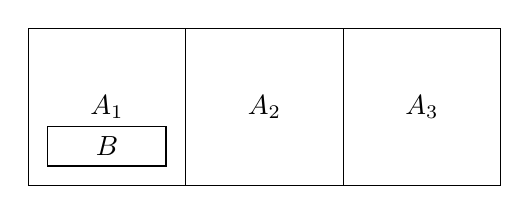
\begin{tikzpicture}
                \draw (0,0) rectangle (2,2) node[pos=0.5]{$A_1$};
                \draw[shift={(2,0)}] (0,0) rectangle (2,2) node[pos=0.5]{$A_2$};
                \draw[shift={(4,0)}] (0,0) rectangle (2,2) node[pos=0.5]{$A_3$};
                \draw (0.25,0.25) rectangle (1.75,0.75) node[pos=0.5]{$B$};
            \end{tikzpicture}
            \caption{Example case for $\mathbb R^2$. We can see that the set $B$ cannot be approximated by the sets $A_1, A_2$ and $A_3$.}
        \end{center}
    \end{figure}
\end{itemize}

\section*{Exercise 3}
\begin{enumerate}
    \item $I_2$ is an open square in $\mathbb R^2$, i.e. a square without its edges.
    \begin{figure}[htbp]
        \centering
        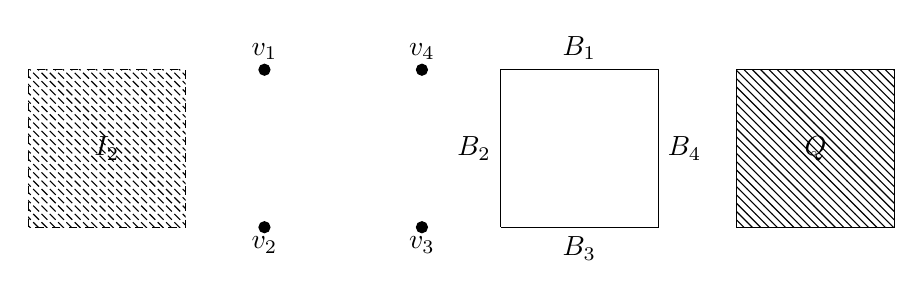
\begin{tikzpicture}
            \draw[dashed, pattern=north west lines, pattern color=black] (0,0) rectangle (2,2) node[pos=.5]{$I_2$};

            \draw[fill=black, shift={(3,0)}] (0,0) circle[radius=2pt] node[anchor=north]{$v_2$};
            \draw[fill=black, shift={(3,0)}] (0,2) circle[radius=2pt] node[anchor=south]{$v_1$};
            \draw[fill=black, shift={(3,0)}] (2,0) circle[radius=2pt] node[anchor=north]{$v_3$};
            \draw[fill=black, shift={(3,0)}] (2,2) circle[radius=2pt] node[anchor=south]{$v_4$};

            \draw[shift={(6,0)}] (0,0)--node[pos=.5, anchor=north]{$B_3$}(2,0)--node[pos=.5, anchor=west]{$B_4$}(2,2)--node[pos=.5, anchor=south]{$B_1$}(0,2)--node[pos=.5, anchor=east]{$B_2$}(0,0) ;

            \draw[pattern=north west lines, pattern color=black, shift={(9,0)}] (0,0) rectangle (2,2) node[pos=0.5]{$Q$};
        \end{tikzpicture}
        \caption{The set $I_2$, the edges of the unit square, the four vertices and $Q=[0,1]^2$.}
    \end{figure}

    First, 
    $$
        Q = [0,1]^2 = I_2 \cup \bigcup_{i=1}^4 v_i \cup \bigcup^4_{i=1} b_i,
    $$ 
    where $v_i \in \{ (0,0),(0,1),(1,0),(1,1) \}$ are the four vertices of the unit square, and $B_i \in \{\{0\} \times ]0,1[, \{1\} \times ]0,1[, ]0,1[ \times \{0\}, ]0,1[ \times \{1\} \}$ are the four edges of the unit square. Now, it holds $\chi(\{v_i\}) = 1$ since $\{v_i\}$ is closed and convex. Additionally, 
    $$
        1 = \chi(\{0\} \times [0,1]) = \chi(B_1) + \chi(\{(0,0)\}) + \chi(\{(0,1)\}) = \chi(B_1) + 1 + 1
    $$ 
    and from this follows $\chi(B_1) = -1$. The same for $B_2, B_3$ and $B_4$.

    So, 
    $$
        1 = \chi(Q) = \chi(I_2) + \underbrace{\sum^4_{i=1}\chi(\{v_i\})}_{=4} + \underbrace{\sum^4_{i=1}\chi(B_i)}_{=-4} 
    $$

    Therfore, $\chi(I_2) = 1$.

    \item Let's compute $\chi(I_3)$, where $I_3$ is the open unit cube in $\mathbb R^3$. The unit cube $Q = [0,1]^3$ has $8$ vertices, and $12$ edges. Each vertex has an Euler characteristic of $1$ and each edge has an Euler characteristic of $-1$. So, $1=\chi(Q) = \chi(I_3) + 8 - 12 \implies \chi(I_3) = 5$.
\end{enumerate}


\section*{Exercise 4}

Let $A_1,...,A_n \subset \mathbb R^d$ be closed and convex such that $B = \bigcap^n_{i=1} A_i \neq \emptyset$. It holds $\chi(B) = 1$, for $B = \bigcap^n_{i=1} A_i$ is closed and convex. Let $\tilde A_0 = B$, $\tilde A_i = A_i \setminus \bigcup^{i-1}_{j=0}\tilde A_{j}$ for $i=1,...,n$. 

Let $[X],[Y] \in \mathcal C(\mathbb R^d)$. First, we want to show that $[X \setminus Y] \in \mathcal C(\mathbb R^d)$. It holds $[X \setminus Y] = [X \cap Y^c] = [X] \cdot (1-[Y]) = [X] - [X] \cdot [Y]$. We showed in exercise 2, that $\mathcal C(\mathbb R^d)$ is closed under multiplication. Consequently, $[X \setminus Y] \in \mathcal C(\mathbb R^d)$.

We see that $\tilde A_i \in \mathcal C(\mathbb R^d)$ for all $i=1,...,n$:
$$
[\tilde A_1] = [A_1 \cap B^c] = [A_1] \cdot (1-[B]) = \underbrace{[A_1]}_{\in \mathcal C(\mathbb R^d)} - \underbrace{[A_1 \cap B]}_{\in \mathcal C(\mathbb R^d)} \in \mathcal C(\mathbb R^d)
$$
$$
    [\tilde A_i] = [A_i \cap \bigcup^{i-1}_{j=0}\tilde A_j] = [A_i \setminus \tilde A_{i-1} \setminus ... \setminus \tilde A_0]
$$
sdad
$$
    [\tilde A_1] = [A_1 \cap B^c] = [A_1] \cdot (1-[B]) = \underbrace{[A_1]}_{\in \mathcal C(\mathbb R^d)} - \underbrace{[A_1 \cap B]}_{\in \mathcal C(\mathbb R^d)} \in \mathcal C(\mathbb R^d)
$$
Now, assume $\tilde A_{i-1} \in \mathcal C(\mathbb R^d)$. Next, we show that $\tilde A_{i} \in \mathcal C(\mathbb R^d)$.
$$
    [\tilde A_i] = [A_i \cap \bigcap^{i-1}_{j=1}\tilde A_{j}^c] = [A_i] \cdot \prod^{i-1}_{j=1}(1-[\tilde A_{j}]) = \underbrace{[A_i]}_{\in \mathcal C(\mathbb R^d)} - \underbrace{[A_i \cap \tilde A_{i-1}]}_{\in \mathcal C(\mathbb R^d)} \in \mathcal C(\mathbb R^d)
$$

Finally, we compute $\chi(\bigcup A_i) = \chi(\bigcup \tilde A_i)$. Note that $\chi(\tilde A_1) = \chi(A_1) - \chi(B) = 1 - 1 = 0$. Assume that $\chi(\tilde A_{i-1}) = 0$. Then, $\chi(\tilde A_i) = \chi(A_i) - \chi(\tilde A_{i-1}) = 1 $



\end{document}